Le petit théorème de Fermat permet assez simplement de déterminer si un nombre est premier ou non. Cependant le processus peut prendre un certain temps.\\

\subsubsection{Fonctionnement}

Notre implémentation du petit théorème de Fermat fonctionne avec de l'aléatoire. On tire cinq fois un nombre \textit{a} aléatoire, allant de 1 à $p-1$ où \textit{p} est le nombre dont on souhaite déterminer la primalité. Le nombre de tirages a été choisi arbitrairement, cependant plus celui-ci est élevé moins le théorème se trompe.\\
Une fois le nombre \textit{a} tiré, on effectue un test avec un modulo. Le test est le suivant:\\
\begin{center}
$a^{p-1} \equiv 1$ (mod p)
\end{center}
Si ce test est faux, le nombre n'est pas premier donc on arrête le programme. Si il est juste, on continue avec de nouvelles valeurs pour \textit{a}. Si aucun des tests ne renvoie faux, le nombre a de très grandes chances d'être premier.

\newpage
\subsubsection{Benchmark}

Les captures suivantes montrent le temps de calcul de notre test de primalité basé sur le petit théorème de Fermat pour les nombres suivants: 733, 8 923, 109 547, 3 000 000 et 9 999 991.\\

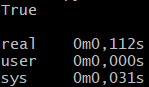
\includegraphics[scale=1]{images/fermat1.png}
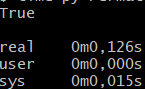
\includegraphics[scale=1]{images/fermat2.png}
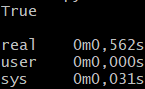
\includegraphics[scale=1]{images/fermat3.png}
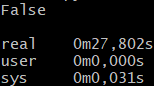
\includegraphics[scale=1]{images/fermat4.png}
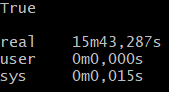
\includegraphics[scale=1]{images/fermat5.png}
\\
Comme on peut le constater, le temps de calcul augmente très rapidement et devient vite trop important avec 15 minutes pour 9 999 991. Il est rapidement trop long de tester la primalité d'un nombre. C'est pourquoi nous avons mis en place une fonction d'exponentiation modulaire.